\chapter{Introduction and Nomenclature}
\label{c:nomenclature}

%------------------------------------------------------------------------
\section{The Known Universe}

Some definitions:
\begin{description}
\item[Model Lattice]
The \vn{model} of the lattice specifies how all the elements are laid
out and what strengths the components have.
\item[Design Lattice] 
The \vn{design} lattice is the particular model lattice that one wants the
machine to conform to.
\item[Base Lattice]
It is sometimes
convenient to designate a reference model lattice so that changes in the
\vn{model} from the reference point can be looked at.  This reference model
is called \vn{base}.
\item[Data] 
Each data point (for example, the horizontal orbit at some
detector) has a number of quantities associated with it:
\begin{description}
\item[Measured Data] 
The data obtained from some measurement. This is generally referred to
as just \vn{data}. When doing lattice design the \vn{data} corresponds to
a constraint (see below).
\item[Reference Data] 
Reference data obtained from some measurement.
\item[Model Data]
The data as calculated from the \vn{model} lattice.
\item[Design Data]
The data as calculated from the \vn{design} lattice.
\item[Base Data]
The data as calculated from the \vn{base} lattice.
\end{description}
\item[Variable]
Since certain variables in the \vn{model} get used often it is
convenient to have lists of these variables that one can refer to. For
example, it is typically convenient to have a list for the variables
that correspond to the strengths of the horizontal steering elements
used to correct the closed orbit.
Each variable has a number of values associated with it:
\begin{description}
\item[Measured Value] 
The Value as obtained at the time of the \vn{data} measurement.
\item[Reference Value] 
The Value as obtained at the time of the \vn{reference} data  measurement.
\item[Model Value]
The value as given in the \vn{model} lattice.
\item[Design Value]
The value as given in the \vn{design} lattice.
\item[Base Value]
The value as given in the \vn{base} lattice.
\end{description}
\end{description}

Blocks of like data are associated with what are called \vn{d1_data}
structures and sets of \vn{d1_data} structures are collected into what
are called \vn{d2_data} structures. For example, a \vn{d1_data}
structure is typically associated with the horizontal data and another
\vn{d1_data} structure is typically associated with the vertical orbit
data. These two structures are then collected into a \vn{d2_data}
structure representing all orbit data. The \vn{d1_data} and
\vn{d2_data} structures are defined in the \tao initialization file
(cf.~Chapter~\ref{c:init}).  When issuing \tao commands one can
specify all the data associated with a \vn{d2_data} structure use the
structure's \vn{class}.  For example the name \vn{orbit} specifies the
orbit data. To specify the data associated with a \vn{d1_data}
structure use the format \vn{class:sub_class} where \vn{sub_class} is the
\vn{sub_class} name of the \vn{d2_data} structure. For example, the horizontal
orbit data is specified by the name \vn{orbit:x}.

Blocks of variables are also associated with what is called a
\vn{v1_var} structure and each of these structures has a \vn{class}
name with which to refer to them in \tao commands.

The \vn{model}, \vn{design}, \vn{base} lattices along with any
\vn{data} and \vn{variables} and their associated structures are
bundled together to form what is called a \vn{universe}. \tao can
simultaneously handle multiple universes. Why is this useful? It can
be used, for example, to simulate both rings of a collider
machine. This can be convenient if there are, say, steering elements
in common and it is needed to simultaneously correct the orbit in both
rings. Another example is in a machine where orbits have been measured
under different conditions of, say, beam energy, and it is desired to
fit all the data simultaneously to try to find, say, rolls in the
bends.

%------------------------------------------------------------------------
\section{Lattice Corrections}

Examples of lattice corrections include flattening the orbit and
adjusting quadrupoles to correct the measured betatron phase. The
general idea is to vary an appropriate set of \vn{variables} with the
aim of minimizing a merit function \vn{M} that is a measure of how well the
model data fits the measured data
\Begineq
  {\cal M} = \sum_{\data:i} w_i 
    (\data\_\model(i) -  \data\_\meas(i))^2 + 
  \sum_{\var:j} w_j 
    (\var\_\model(j) - \var\_\meas(j))^2
  \label{m1}
\Endeq
\vn{data_model} is data as calculated from the model and
\vn{data_meas} is the actual measured data. \vn{var_model} is the
value of a variable in the \vn{model} and \vn{var_meas} is the value
as measured at the time the data was taken. The second term in the
merit function helps prevent degeneracies, or near degeneracies,
allowing \tao to find solutions where \vn{data_model} matches
\vn{data_measured} with the \vn{var_model} having ``unphysical''
values. The weights \vn{w_i} and \vn{w_j} need to be set depending
upon how accurate the data is and how accurate the calibrations for
measuring the \vn{var_measured} values are. With the second term in
the merit function the number of constraints (number of terms in the
merit function) is always larger than the number of variables so
degeneracies can never appear. The algorithm used for minimizing
\vn{M} is called an \vn{optimizer} and the \vn{run} command is used to
invoke a, \vn{optimizer}.

presumably, once a ``fit'' has been made, by varying the appropriate
\vn{variables} in the \vn{model} to minimize the merit function, the
model values of the \vn{variables} are the true values that existed
when the measurement is taken. Thus, if \vn{M} is reasonably small we 
believe:
\begin{example}
  var_model = var_actual
\end{example}
What is wanted is to have the \vn{variable} values equal to the
design. Therefore, to correct the lattice, the \vn{variables} need to
be changed by
\begin{example}
  var_change = var_final  - var_start
             = var_design - var_model
\end{example}
In other words
\begin{example}
  var_final = var_start + (var_design - var_model)
\end{example}
Notice that the fitting process is independent of the \vn{design}
lattice. It is only when calculating the corrections to the
\vn{variables} that the \vn{design} lattice plays a roll. 

Sometimes it is desired to fit to changes in data as opposed to the
absolute value of the data. For example, when closing an orbit bump
knob what is important is the difference in orbits before and
after the bump knob is varied. In this case the merit function becomes
\begin{alignat}{1}
  {\cal M} = &\sum_{\data:i} w_i 
    \left[ (\data\_\model(i) - \data\_\design(i)) - 
      (\data\_\meas(i) - \data\_\reference(i)) \right]^2 + \CRNO
  &\sum_{\var:j} w_j 
    \left[ (\var\_\model(j) - \var\_\design(j)) -
     (\var\_\meas(i) - \var\_\reference(i)) \right]^2 
  \label{m2}
\end{alignat}
This merit function is acceptable if the reference data is taken with
the machine reasonably near the design setup so that nonlinearities
can be ignored. If this is not the case then the fitting becomes a two
step process: The first step is to fit the \vn{model} to the \vn{reference}
data using the merit function of \Eq{m1}. The \vn{base} lattice is then
set equal to the \vn{model} lattice. The second
step is to fit the model using the merit function
\begin{alignat}{1}
  {\cal M} = &\sum_{\data: i} w_i 
    \left[ (\data\_\model(i) - \data\_\base(i)) - 
      (\data\_\meas(i) - \data\_\reference(i)) \right]^2 + \CRNO
  &\sum_{\var: j} w_j 
    \left[ (\var\_\model(j) - \var\_\base(j)) -
     (\var\_\meas(i) - \var\_\reference(i)) \right]^2 
  \label{m3}
\end{alignat}

Control of what data and what variables are to be used in the fitting
process is controlled by the \vn{use}, \vn{veto}, \vn{restore}, and
\vn{clip} commands.

%------------------------------------------------------------------------
\section{Lattice Design}

Lattice design is the process of calculating \vn{variable} strengths
to meet a number of criteria (called constraints). For example, one
constraint could be that the beta function in some part of the lattice
not exceed a certain value. In this case we can proceed as was done
for lattice correction and define a merit function to be minimized:
\Begineq
  {\cal M} = \sum_{\mbox{constraints} i} w_i \, C_i^2
\Endeq
\vn{C_i} is the constraint value which is dependent upon the \vn{class} of
the constraint:
\begin{description}
\item[target]
\Begineq
  C = (\mbox{Model} - \mbox{Target})
\Endeq
\item[min]
\Begineq
  C = 
    \begin{cases}
    0                               & \mbox{Model} > \mbox{Target} \\
    (\mbox{Model} - \mbox{Target})  & \mbox{Model} < \mbox{Target} 
    \end{cases}
\Endeq
\item[max]
\Begineq
  C = 
    \begin{cases}
    (\mbox{Model} - \mbox{Target})  & \mbox{Model} > \mbox{Target} \\ 
    0                               & \mbox{Model} < \mbox{Target}
    \end{cases}
\Endeq
\end{description}

%------------------------------------------------------------------------
\section{Plotting}

Some definitions:
\begin{description}
\item[Curve]
A \vn{curve} is a set of (x,y) points to be plotted.
\item[Graph]
A \vn{graph} consists of horizontal and vertical axes along with a set
of \vn{curve}s that are plotted within the graph. 
\item[Plot]
A \vn{plot} is essentially a collection of \vn{graphs}.
\item[Page]
The \vn{page} refers to the x--window where graphics are displayed or the 
corresponding printed graphics page.
\item[Region]
The \vn{page} is divided up into a number of \vn{region}s. 
\end{description}

\begin{figure}
  \centering
  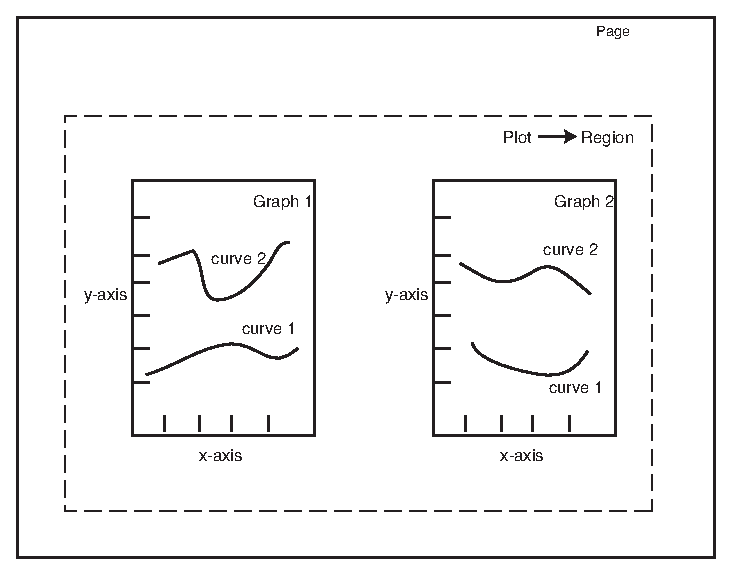
\includegraphics{plot.psfig}
  \caption{A plot has is a collection of graphs and a graph has a 
collection of curves. A plot becomes visible when it 
is associated with a region using the \vn{place} command.}
  \label{f:plot}
\end{figure}

The plot initialization file (cf.~Chapter~\ref{c:init}) defines a set
of \vn{template} plots. A \vn{template} defines what class of data is
plotted (orbit, coupling, etc.), how many \vn{graphs} there are, what
the scales are for the \vn{graph} axes, how the \vn{graph}s are laid
out, etc.  The plot initialization file also defines a set of
\vn{region}s within the \vn{page}.  Using the \vn{place} command one
can assign a particular template to a particular region for plotting.
The relationship between \vn{region}, \vn{plot}, \vn{graph}, and
\vn{curve} is shown graphically in Figure~\ref{f:plot}.

Using the \vn{plot} command one can then specify \vn{who} is
plotted. \vn{who} refers to \vn{measured}, \vn{reference}, \vn{model},
\vn{base}, and/or \vn{design} data.  Notice that the same \vn{template}
plot can be assigned to different \vn{regions} and the plots in different
\vn{regions} can have different scales for their axes or different
\vn{who}.


The \vn{use}, \vn{veto}, \vn{restore},
and \vn{clip} commands are used to display or not to display
individual data points. These are the same commands that control what
data is used in fitting the model to the data. The general rule is
that data that is vetoed for display are simultaneously vetoed for fitting.

When issuing \tao commands, to specify a particular \vn{graph} in a plot
use the notation:
\begin{example}
  region:graph
\end{example}
For example, If a template has two graphs named \vn{x} and \vn{y} and
this template is assigned to the \vn{top} region then the \vn{x} graph
is referred to as \vn{top:x}. 

